\section{Ingående system}
Svävaren har flertalet olika delsystem och i figur \ref{fig:Systemskiss} så ser
man hur de olika delarna är sammankopplade. Blocken som i figuren kallas
fjärrkontroll och Android är två separata Androidplattformar. Det senare kommer
i fortsättningen av rapporten att kallas för Router, då det är det som den har
som huvuduppgift.

\begin{figure}[htbp!] 
\centering 
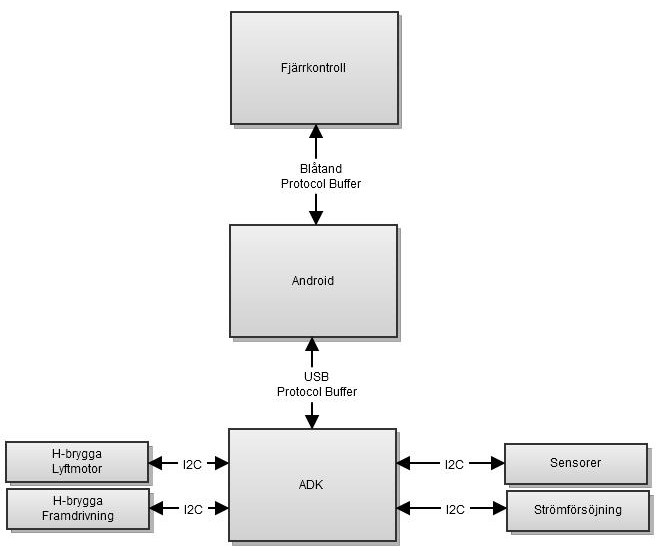
\includegraphics[width=13cm]{../includes/figures/Systemskiss} 
\caption{Systemskiss över svävaren.} 
\label{fig:Systemskiss} 
\end{figure}

Att arbeta med Android som bas för plattformar valdes för att mycket
funktionalitet fås till ett billigt pris. Ur ett
hårdvaruperspektiv så ingår det ett flertal sensorer och kommunikationskanaler
som är användbara vid utveckling av en radiostyrd enhet.

I kommande underavdelingar finns mer detaljerad information om varje delsystem.
\subsection{ADK}
Rickard\ldots
\subsection{Fjärrkontroll}
Som nämnt i avsnitt \ref{subsec:system/fjarrkontroll} så har Fjärrkontrollen tre
stora uppgifter: generera styrsignaler till svävaren, kommunicera med de andra
enheterna samt att kunna logga händelser på svävaren.

Applikationen är uppdelad tre huvudsakliga delar som var och en utgörs av en
Android-service. Dessa delar implementerar funktionalitet för kommunikation,
loggning av sensordata samt generering av styrsignaler. Applikationen innehåller
även Android-activity som fungerar som inställningsmeny för fjärrkontrollen.

Genomgång på hur kommunikationen mellan fjärrkontrollen och de andra enheterna
sker gås igenom i avsnitt \ref{subsec:commlink} och generering av
styrsignaler behandlas i \ref{subsec:styr och regler}. Nedan beskrivs hur
loggning fungerar.

\subsubsection{Loggning av sensordata}
Funktionaliteten för att logga olika typer av sensordata sker genom att kryssa
i vilka sensorer som data ska sparas i från. Insamlade data sparas som textfiler
på fjärrkontrollens SD-minne.
På den senaste versionen av applikationen finns funktionalitet för loggning av
data från fjärrkontrollens accelerometer, svävarens accelerometer samt från
svävarens ultraljudssensorer. Vilken data som skall loggas ställs in i
inställningsmenyn. Om data från svävaren önskas skickas ett kommando till den
som gör att den svarar med ett paket innehållande önskad data.

\subsubsection{Resultat}
Fjärrkontrollen möter de krav som ställs i kravspecifikationen. Vid skrivandet
av rapporten hade tester dock bara genomförts på plattformar av
smartphone-modell.

\begin {itemize}
\item Räckvidd 20 meter
\item Indikera när kommunikationen med svävaren bryts.
\item Kunna kommunicera med svävaren. Samt ge de kommandon som gränssnittet till
svävaren tillåter.
\end {itemize}

\subsubsection{Vidareutveckling}
Som brukligt så blir man aldrig riktigt klar med utveckling av mjukvara, det
finns alltid saker att finslipa. Loggningsfunktionen bör kontrolleras noggrant
och utökas så att fler sensorer går att logga. Protocol Buffer är inte
implementerat som protokoll och det skulle med relativ enkelhet kunna ändras.

\subsection{Router}
Routerns uppgifter är att handha reglersystemet och att agera som
kommunikationslänk mellan de olika enheterna.

Programmet är indelat i tre Android-services och en Android-activity:
\begin{itemize}
	\item Bluetoothservice som hanterar all Bluetoothkommunkation,
	\item UsbService som hanterar all USBkommunkation,
	\item ControlSystemService som implementerar reglersystemet
	\item och MainActivity som implementerar användargränssnittet.
\end{itemize}

Applikationen startas automatiskt genom att ansluta ADK:n till router-telefonen. 
Om applikationen körs innan den ansluts till ADK:n kommer den att startas om för
att upprätta USB-kommunikationen.
När appen körs visas en diod för respektive kommunkationsbuss. Om kommunkationen
fungerar lyser dioden grönt och om den inte fungerar så lyser den rött. Dioden
kan även lysa gult men detta är inget man hinner se i vanliga fall då den enbart
gör så under uppkoppling. Knappen "Bluetooth setup" används för att upprätta en
Bluetoothlänk.

Intern kommunkation inom applikationen sker via Android Broadcasts.
Kommunikationen med andra enheter behandlas i avsnitt \ref{subsec:commlink} och
reglersystemet behandlas i \ref{subsec:styr och regler}.

\subsubsection{Resultat}
Programmet är stabilt och uppfyller alla krav. Dess huvudsyfte är att ta emot
och skicka vidare meddelanden vilket fungerar utmärkt.
\subsection{H-brygga}
\ldots
\subsection{Motorer och fläktar}
De lyftfläktar som används är fyra stycken centrifugalfläktar som generellt sett
inte ger lika mycket luftflöde som axiella fläktar men ger däremot mycket högre
lufttryck istället. Genom att placera de fyra fläktarna parallellt med varandra
blir luftflödet ungefär fyra gånger större än för en fläkt och ger därmed ett
tillräckligt luftflöde. Ett högt lufttryck ger bidrag till att svävaren kan bära
en större totalvikt. Se specifikation av centrifugalfläkten i Tabell
\ref{tbl:fan_spec} och se mer information i datablad \cite{Delta_BFB1212VH-R00}
. Mer information kring hur lyftkraftsberäkningarna gjordes fås i Appendix
\ref{app:lyftkraftsberakningar}.

\begin{table}[htbp!]
\centering
\caption{Specifikation av centrifugalfläkt.}
\label{tbl:fan_spec}
\begin{tabular}{|l|r|}
\hline
Märkspänning & 12 V\\
\hline
Driftspänning & 4,0 - 13,8 V\\
\hline
Ström & 1,25 A\\
\hline
Effekt & 15,00 W\\
\hline
Rotationshastighet & 3100 rpm\\
\hline
Maximalt luftflöde & 1,120 m$^3$/min\\
\hline
Maximalt lufttryck & 323,6 Pa (33,00 mmH$_2$O)\\
\hline
Ljudnivå & 56,5 dB-A\\
\hline
\end{tabular}
\end{table}

Till drivningen används två stycken elmotorer (DC) som driver varsin propeller.
Se specifikation av motorn i Tabell \ref{tbl:motor_spec} och se mer information
i datablad, \cite{Motraxx_XFLY400-12}.

\begin{table}[htbp!]
\centering
\caption{Specifikation av elmotor.}
\label{tbl:motor_spec}
\begin{tabular}{|l|r|}
\hline
Märkspänning & 12 V\\
\hline
Driftspänning & 6 - 15 V\\
\hline
Tomgångsvarvtal & 21000 rpm\\
\hline
Tomgångsström & 0,6 A\\
\hline
Maximal effekt & 42,1 W\\
\hline
VID MAXIMAL EFFEKTIVITET &\\
\hline
Lastvarvtal & 19000 rpm\\
\hline
Strömförbrukning & 2,5 A\\
\hline
Vridmoment & 1,00 Nmm\\
\hline
Avgiven effekt & 19,5 W\\
\hline
Effektivitet (verkningsgrad) & 65\%\\
\hline
\end{tabular}	
\end{table}

\subsection{Strömförsörjning}
Strömförsörjningen designades med moduläritet i  åtanke så att flera olika
spänningsnivåer uppnås genom samma design på kretskort. De olika
strömförsörjningskorten som det designades för är:
\begin{itemize}
	\item 3,3 V, 3 A, med en felmarginal på $\pm$0.2 V.
	\item 5 V, 3 A, med en felmarginal på $\pm$0.5 V.
	\item 12 V, 3 A, med en felmarginal på $\pm$0.8 V.
	\item En justerbar spänningsnivå med en felmarginal på $\pm$10 \% av den
önskade spänningen och kunna leverera 3 A.
\end{itemize}

Varje typ av strömförsörjning skulle finnas på ett separat PCB, dock med samma
layout för enkel tillverkning och att eventuell beställning av kort skulle vara
billig.

Strömförsörjningarna designades också så att de gick att parallellkoppla, både
på ingångs- och utgångssidan. Detta för att kunna utöka kapaciteten vid behov.

För att uppnå kraven och för att nå god effektivitet så används switchade
regulatorer, för mer teori och val av design och komponenter se Appendix
\ref{apx:PSU}.

\subsubsection{Resultat}

Totalt 6 stycken strömförsörjningskort används i svävaren och versionerna som
konstruerades är:
\begin{itemize}
\item 2 stycken justerbara 13.8 V som driver lyftfläktarna (ett
strömförsörjningskort till två fläktar).
\item 2 stycken justerbara 10 V för drivning av drivfläktarna (ett
strömförsörjningskort per fläkt).
\item 1 stycke 12 V till drivkretsarna på båda H-bryggorna.
\item 1 stycke 5 V för ADK och logikkretsarna på båda H-bryggorna.
\end{itemize}

Korten klarar av att hålla både ström och spänningsnivåerna bra utan störningar
eller spikar.

\subsubsection{Diskussion}
Då kraven på strömförsörjningen specificerades så var det inte bestämt om det
skulle byggas ett nytt chassi med andra motorer eller inte. Därför så valdes
spännings och strömnivåer från den gamla svävaren som grund och korten
designades därefter. Detta ledde till att det behövdes fler
strömförsörjningskort än planerat. Men det medförde dock inte några problem och
detta tack vare det modulära tänkandet.

Vid för tung belastning, t.ex med starkare motorer och fläktar,
sjunker spänningen och strömmen ökar och därav bör det användas säkringar
på 4-6~A.

Det visade sig att de justerbara spänningsnivå korten var ett mycket bra val, då
vi lätt kunde öka nivån för fläktar och motorer så bäst funktion kunde erhållas.
Vid de högre spänningarna är det värt att notera att det behövdes kylflänsar
på regulatorerna.

Strömförsörjnningskorten har plats för filterkomponenter både innan regulatorn
och efter, dessa platser är i nuläget tomma och förbikopplade då inga större
störningar eller spikar kunnat uppmätas.

\subsubsection{Förbättringar}
I själva designen för strömförsörjningskorten så bör man inkludera en en
diod som förhindrar backspänning från de andra korten som lägger sig
över avstängda kort. Problemet kan återskapas lätt genom att stänga av ett
strömförsörjningskort men att ha det sammankopplat med andra
strömförsörjningskort som är i drift. Då kan statusdioder lysa trots att kortet
är avstängt. Den backspänning som uppkommer gör ingen skada på
strömförsörjningskorten, men det är lite förvillande att ett korts statusdioder
lyser trots att kortet är avstängt. Notera även  att det är H-bryggorna som
bidrar med att denna backspänning uppstår då de har flera spänningar inkopplade.

Då nuvarande strömförsörjning inte klarar att ge mer än 3 A vid sin
spänningsnivå begränsar det, mer än förväntat, val av motorer och fläktar. Så
ett strömförsörjningskort designat för högre ström skulle vara en klar
förbättring. Detta skulle också minska antalet strömförsörjningskort.
För detta kort rekommenderas det att man ej använder en färdig regulator utan
själv bygger upp det för att få bra funktion och strömbegrännsning.

\newpage
\subsubsection{Ekonomi}
Kostnad för komponenterna för de olika spänningsnivåerna ses i tabellerna \ref{gemensammadelar} - \ref{justerbar}.

\begin{table}[htbp]
\centering
\caption{Gemensamma delar}
\begin{tabular}{|l|l|r|r|}
\hline
\textbf{Komponent} & \textbf{Information} & \textbf{Antal} & \textbf{Pris} \\ 
\hline
Kondensator & 680uF, 35V & 1 & 5,68 \\ 
\hline
Schottky diod & SB540 & 1 & 6,05 \\ 
\hline
Tryckvippströmställare & R19U-R112A-B-2-B-M2 & 1 & 9,03 \\ 
\hline
Molex hane & 2p & 2 & 4,56 \\ 
\hline
Stiftdon 90\degree & 2p & 2 & 9,86 \\ 
\hline
Säkringshållare & 6,3A & 2 & 3,07 \\ 
\hline
Lysdiod & 1224-10SYGC/S530-E2 & 2 & 1,49 \\ 
\hline
\textbf{Total} &  & \multicolumn{1}{l|}{} & 39,74 \\ \hline
\end{tabular}
\label{gemensammadelar}
\end{table}


\begin{table}[htbp]
\centering
\caption{5~V Strömförsörjning}
\begin{tabular}{|l|l|r|r|}
\hline
\textbf{Komponent} & \textbf{Information} & \textbf{Antal} & \textbf{Pris} \\
\hline
Switch regulator, 5V, TO-220  & LM2596T33 & 1 & 52,62 \\ 
\hline
Spole &  47 UH  & 1 & 16,73 \\ 
\hline
Kondensator & 330UF, 35V & 1 & 5,86 \\ 
\hline
\textbf{Total} &  & \multicolumn{1}{l|}{} & 114,95 \\ 
\hline
\end{tabular}
\label{5vstrom}
\end{table}


\begin{table}[htbp]
\centering
\caption{12~V Strömförsörjning}
\begin{tabular}{|l|l|r|r|}
\hline
\textbf{Komponent} & \textbf{Information} & \textbf{Antal} & \textbf{Pris}  \\ 
\hline
Switch regulator, 12V, TO-220  & LM2596T-12  & 1 & 59,58 \\ 
\hline
Spole & 47 uH  & 1 & 16,73 \\ 
\hline
Kondensator & 180UF, 35V & 1 & 2,33 \\ 
\hline
\textbf{Total} &  & \multicolumn{1}{l|}{} & 118,38 \\ 
\hline
\end{tabular}
\label{12vstrom}
\end{table}


\begin{table}[htbp!]
\centering
\caption{Justerbar spänning strömförsörjning}
\begin{tabular}{|l|l|r|r|}
\hline
\textbf{Komponent} & \textbf{Information} & \textbf{Antal} & \textbf{Pris} \\
\hline
Switch regulator, justerbar, TO-220  & LM2596T-ADJ  & 1 & 56,73 \\ 
\hline
Spole  & 68uH & 1 & 16,73 \\ 
\hline
Kondensator & 220UF, 35V  & 1 & 3,91 \\ 
\hline
\textbf{Total} &  & \multicolumn{1}{l|}{} & 117,11 \\ 
\hline
\end{tabular}
\label{justerbar}
\end{table}

Även dessa kort beställdes från ITead Studio för en kostnad av 369,50 SEK, vilket ger en sammanlagd summa av 759,68 SEK för alla strömförsörjningskort.




\subsection{Batterier}
En studie av olika batteritekniker gjordes för att se vilka som skulle klara
kraven. Valet föll på LiPo-tekniken, då denna har hög effektdensitet och är
kostnadseffektiv.

\subsubsection{Resultat}
Två stycken 5 cells LiPo-batterier på 18,5 V och 3.3 Ah används, där ett går
till enbart strömförsörjningen för lyftfläktarna (då dessa kräver högst spänning
och mest ström) och det andra till resterande elektronik. Batteriernas
specifikation kan läsas i Tabell \ref{tbl:Battery}.

\begin{table}[htbp!]
\centering
\caption{Batterispecifikation}
\label{tbl:Battery}
\begin{tabular}{l|l}
Egenskap & Värde \\
\hline
Minsta strömkapacitet & 3300 mAh\\
Konfiguration & 5S1P / 18.5V / 5Cell\\
Maximal konstant urladdning & 30C\\
Maximal toppurladdning (10 s) & 40C\\
Vikt & 480g\\
Dimensioner (l * b * h) & 139 mm * 43 mm * 35mm\\
\end{tabular}
\end{table}

Spänningsnivån på 18,5 V är framförallt på grund av att regulatorn på
strömförsörjningskortet behöver ha minst 15 V in för att kunna hålla 12 V eller
högre ut. 3.3 Ah för att klara kraven på 10 minuters drifttid vid max
påfrestning. Inget test av maximal drifttid har gjorts men tester med minst 30
minuters körning klarades.

\subsubsection{Diskussion}
Batterierna mötte kraven väl. Eventuellt så skulle man kunna minska
strömkapaciteten för att minska totalvikten på svävaren. Projektgruppen tyckte
inte att den extra kostnaden, både i tid och pengar, samt
att försämringen av prestandan var värd inköp av andra batterier.

\subsubsection{Ekonomi}
Inköpet av batterier kostade 979 SEK, inklusive tull och frakt.

\subsection{Chassi}
Vid design av chassit användes CAD-programmet SolidWorks 2012 för att göra
3D-modeller över chassits olika delar. En prototyp modellerades i SolidWorks och
tillverkades för att användas till olika tester innan det slutliga chassit
skulle designas och tillverkas.

\subsubsection{Material}
Chassit är gjort av ett lätt skivmaterial som består av två tunna “pappskivor”
med skumplast emellan. Skivorna är 3,1 mm tjocka och är lätta att klippa, skära
och limma. Skivorna skänktes till projektgruppen av Björn-Åke
Sköld för att göra en prototyp av svävaren. Materialet användes till prototypen
men även till den slutliga svävaren.

Dysorna till fläktarna är gjorda av gjutrör av papp  och träramen som håller
ihop höljet som döljer elektroniken är av furu. Till kjolen användes ett
ripstop-tyg som är ett slitstarkt tunt tyg som används bl.a. till drakar.

\subsubsection{Prototyp}
Arbetet inleddes med att göra en CAD-modell över prototypen. Den gjordes dubbelt
så stor jämfört med den svävare som en tidigare projektgrupp har byggt.
Björn-Åke trodde nämligen att man skulle kunna göra en lite större svävare men
som ändå är lättare än den gamla vid användning av hans material.

Prototypen blev 800x570 mm och 100 mm hög. Tanken var att den gamla svävaren
skulle fästas ovanpå prototypen för att se om den kunde lyfta och sväva då. En annan tanke var
att även kjolen skulle ha testats på prototypen för att sedan kunna flyttas över
till den slutliga svävaren. Eftersom det inte skulle bli helt lätt att fästa den
gamla svävaren på prototypen testades prototypen direkt med de lyftfläktar som
skulle användas. Den kunde då lyfta och hållas svävande trots att ingen kjol
användes. Kjolen designades som en variant av fingerkjol bestående av flera
segment men hann inte sys innan en idé på en ny design dök upp.

\subsubsection{Ny design}
Efter ett möte med Björn-Åke, då han fick se prototypen och CAD-modellen av
kjolen, bestämdes att både chassit och kjolen skulle konstrueras om. Detta för
att kjolsegmenten blev för små att sy och att kjolen i sin helhet inte skulle
kunna hålla kvar luften så att ett lufttryck kunde erhållas.

I den nya designen
kunde höjden halveras på svävaren och bredden ökas 3 cm, detta för att göra
sävaren stabilare. Det nya chassit har en bagkjol istället
eftersom det är lättare att sy en sådan kjol och den kan dessutom hålla kvar
luften på ett bättre sätt så ett lufttryck erhålls. En bagkjol är inte lika
flexibel som en fingerkjol när det gäller att ta sig över hinder men i detta
projekt är bagkjolen tillräckligt flexibel.

Kjolen sitter fast i en plattform med kardborreband och eftersom det försvinner
mycket luft vid kardborrefästena har inte några hål gjorts i kjolen. På så vis
erhålls även ett lufttryck i kjolen som gör att svävaren kan bära en större
totalvikt.

Plattformen som kjolen är fäst runt är 800x600 mm och består av två
plattor av det lätta skivmaterialet. Den undre plattan är lite mindre än den
övre och de sitter ihop med distanser för att få en luftspalt på 10 mm mellan
plattorna.

En träram konstruerades för att kunna fästa fläktar, motorer och elektronik
i. Den sitter fast i plattformen med kardborreband och håller även ihop höljet
som döljer elektroniken med kardborreband.

Svävaren är uppbyggd på ett modulärt sätt och de olika delarna är placerade på
ett sätt som ger låg tyngdpunkt. Den är även uppbyggd symmetriskt med en jämn
viktfördelning över hela svävarens bottenyta. En 3D-modell över svävaren visas i
Figur \ref{fig:CAD_Hover}.

\begin{figure}[htbp!] 
\centering 
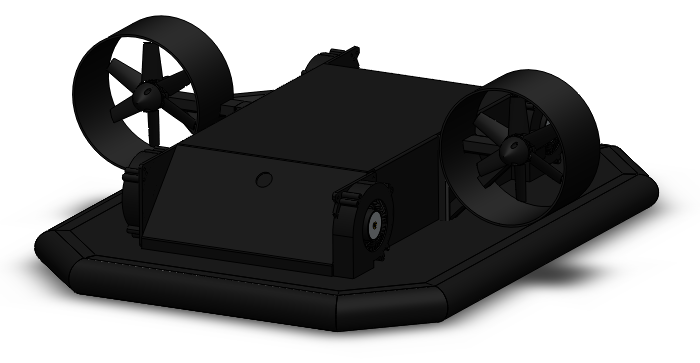
\includegraphics[width=8cm]{../includes/figures/CAD_Hovercraft.png} 
\caption{3D-modell över svävaren.} 
\label{fig:CAD_Hover} 
\end{figure}

\subsubsection{Vidareutveckling}
I en vidareutveckling av svävaren skulle materialet kunna bytas ut mot ett mer
hållbart och vattentåligt material. Skivmaterialet har en tendens att slitas
sönder när delarna ska tas isär vid kardborrefästena.

Träramen som är av furuskulle kunna bytas ut till ett lättare träslag som
balsaträ eller ett annat lätt material.

Genom att skala upp modellen kan en större svävare göras med samma design. Men
det som behöver tänkas på då är att de fläktar och motorer som väljs klarar av
den nya vikten.
